\documentclass[1p]{elsarticle_modified}
%\bibliographystyle{elsarticle-num}

%\usepackage[colorlinks]{hyperref}
%\usepackage{abbrmath_seonhwa} %\Abb, \Ascr, \Acal ,\Abf, \Afrak
\usepackage{amsfonts}
\usepackage{amssymb}
\usepackage{amsmath}
\usepackage{amsthm}
\usepackage{scalefnt}
\usepackage{amsbsy}
\usepackage{kotex}
\usepackage{caption}
\usepackage{subfig}
\usepackage{color}
\usepackage{graphicx}
\usepackage{xcolor} %% white, black, red, green, blue, cyan, magenta, yellow
\usepackage{float}
\usepackage{setspace}
\usepackage{hyperref}

\usepackage{tikz}
\usetikzlibrary{arrows}

\usepackage{multirow}
\usepackage{array} % fixed length table
\usepackage{hhline}

%%%%%%%%%%%%%%%%%%%%%
\makeatletter
\renewcommand*\env@matrix[1][\arraystretch]{%
	\edef\arraystretch{#1}%
	\hskip -\arraycolsep
	\let\@ifnextchar\new@ifnextchar
	\array{*\c@MaxMatrixCols c}}
\makeatother %https://tex.stackexchange.com/questions/14071/how-can-i-increase-the-line-spacing-in-a-matrix
%%%%%%%%%%%%%%%

\usepackage[normalem]{ulem}

\newcommand{\msout}[1]{\ifmmode\text{\sout{\ensuremath{#1}}}\else\sout{#1}\fi}
%SOURCE: \msout is \stkout macro in https://tex.stackexchange.com/questions/20609/strikeout-in-math-mode

\newcommand{\cancel}[1]{
	\ifmmode
	{\color{red}\msout{#1}}
	\else
	{\color{red}\sout{#1}}
	\fi
}

\newcommand{\add}[1]{
	{\color{blue}\uwave{#1}}
}

\newcommand{\replace}[2]{
	\ifmmode
	{\color{red}\msout{#1}}{\color{blue}\uwave{#2}}
	\else
	{\color{red}\sout{#1}}{\color{blue}\uwave{#2}}
	\fi
}

\newcommand{\Sol}{\mathcal{S}} %segment
\newcommand{\D}{D} %diagram
\newcommand{\A}{\mathcal{A}} %arc


%%%%%%%%%%%%%%%%%%%%%%%%%%%%%5 test

\def\sl{\operatorname{\textup{SL}}(2,\Cbb)}
\def\psl{\operatorname{\textup{PSL}}(2,\Cbb)}
\def\quan{\mkern 1mu \triangleright \mkern 1mu}

\theoremstyle{definition}
\newtheorem{thm}{Theorem}[section]
\newtheorem{prop}[thm]{Proposition}
\newtheorem{lem}[thm]{Lemma}
\newtheorem{ques}[thm]{Question}
\newtheorem{cor}[thm]{Corollary}
\newtheorem{defn}[thm]{Definition}
\newtheorem{exam}[thm]{Example}
\newtheorem{rmk}[thm]{Remark}
\newtheorem{alg}[thm]{Algorithm}

\newcommand{\I}{\sqrt{-1}}
\begin{document}

%\begin{frontmatter}
%
%\title{Boundary parabolic representations of knots up to 8 crossings}
%
%%% Group authors per affiliation:
%\author{Yunhi Cho} 
%\address{Department of Mathematics, University of Seoul, Seoul, Korea}
%\ead{yhcho@uos.ac.kr}
%
%
%\author{Seonhwa Kim} %\fnref{s_kim}}
%\address{Center for Geometry and Physics, Institute for Basic Science, Pohang, 37673, Korea}
%\ead{ryeona17@ibs.re.kr}
%
%\author{Hyuk Kim}
%\address{Department of Mathematical Sciences, Seoul National University, Seoul 08826, Korea}
%\ead{hyukkim@snu.ac.kr}
%
%\author{Seokbeom Yoon}
%\address{Department of Mathematical Sciences, Seoul National University, Seoul, 08826,  Korea}
%\ead{sbyoon15@snu.ac.kr}
%
%\begin{abstract}
%We find all boundary parabolic representation of knots up to 8 crossings.
%
%\end{abstract}
%\begin{keyword}
%    \MSC[2010] 57M25 
%\end{keyword}
%
%\end{frontmatter}

%\linenumbers
%\tableofcontents
%
\newcommand\colored[1]{\textcolor{white}{\rule[-0.35ex]{0.8em}{1.4ex}}\kern-0.8em\color{red} #1}%
%\newcommand\colored[1]{\textcolor{white}{ #1}\kern-2.17ex	\textcolor{white}{ #1}\kern-1.81ex	\textcolor{white}{ #1}\kern-2.15ex\color{red}#1	}

{\Large $\underline{12n_{0335}~(K12n_{0335})}$}

\setlength{\tabcolsep}{10pt}
\renewcommand{\arraystretch}{1.6}
\vspace{1cm}\begin{tabular}{m{100pt}>{\centering\arraybackslash}m{274pt}}
\multirow{5}{120pt}{
	\centering
	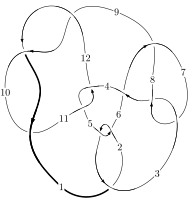
\includegraphics[width=112pt]{../../../GIT/diagram.site/Diagrams/png/2424_12n_0335.png}\\
\ \ \ A knot diagram\footnotemark}&
\allowdisplaybreaks
\textbf{Linearized knot diagam} \\
\cline{2-2}
 &
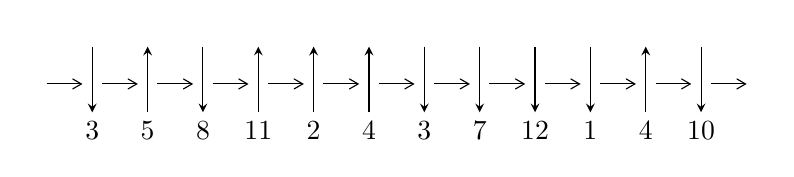
\begin{tikzpicture}[x=20pt, y=17pt]
	% nodes
	\node (C0) at (0, 0) {};
	\node (C1) at (1, 0) {};
	\node (C1U) at (1, +1) {};
	\node (C1D) at (1, -1) {3};

	\node (C2) at (2, 0) {};
	\node (C2U) at (2, +1) {};
	\node (C2D) at (2, -1) {5};

	\node (C3) at (3, 0) {};
	\node (C3U) at (3, +1) {};
	\node (C3D) at (3, -1) {8};

	\node (C4) at (4, 0) {};
	\node (C4U) at (4, +1) {};
	\node (C4D) at (4, -1) {11};

	\node (C5) at (5, 0) {};
	\node (C5U) at (5, +1) {};
	\node (C5D) at (5, -1) {2};

	\node (C6) at (6, 0) {};
	\node (C6U) at (6, +1) {};
	\node (C6D) at (6, -1) {4};

	\node (C7) at (7, 0) {};
	\node (C7U) at (7, +1) {};
	\node (C7D) at (7, -1) {3};

	\node (C8) at (8, 0) {};
	\node (C8U) at (8, +1) {};
	\node (C8D) at (8, -1) {7};

	\node (C9) at (9, 0) {};
	\node (C9U) at (9, +1) {};
	\node (C9D) at (9, -1) {12};

	\node (C10) at (10, 0) {};
	\node (C10U) at (10, +1) {};
	\node (C10D) at (10, -1) {1};

	\node (C11) at (11, 0) {};
	\node (C11U) at (11, +1) {};
	\node (C11D) at (11, -1) {4};

	\node (C12) at (12, 0) {};
	\node (C12U) at (12, +1) {};
	\node (C12D) at (12, -1) {10};
	\node (C13) at (13, 0) {};

	% arrows
	\draw[->,>={angle 60}]
	(C0) edge (C1) (C1) edge (C2) (C2) edge (C3) (C3) edge (C4) (C4) edge (C5) (C5) edge (C6) (C6) edge (C7) (C7) edge (C8) (C8) edge (C9) (C9) edge (C10) (C10) edge (C11) (C11) edge (C12) (C12) edge (C13) ;	\draw[->,>=stealth]
	(C1U) edge (C1D) (C2D) edge (C2U) (C3U) edge (C3D) (C4D) edge (C4U) (C5D) edge (C5U) (C6D) edge (C6U) (C7U) edge (C7D) (C8U) edge (C8D) (C9U) edge (C9D) (C10U) edge (C10D) (C11D) edge (C11U) (C12U) edge (C12D) ;
	\end{tikzpicture} \\
\hhline{~~} \\& 
\textbf{Solving Sequence} \\ \cline{2-2} 
 &
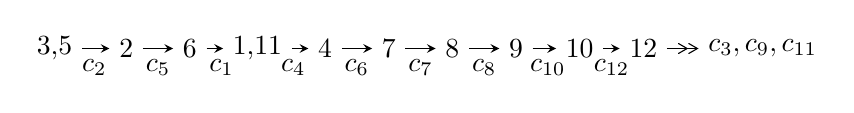
\begin{tikzpicture}[x=23pt, y=7pt]
	% node
	\node (A0) at (-1/8, 0) {3,5};
	\node (A1) at (1, 0) {2};
	\node (A2) at (2, 0) {6};
	\node (A3) at (49/16, 0) {1,11};
	\node (A4) at (33/8, 0) {4};
	\node (A5) at (41/8, 0) {7};
	\node (A6) at (49/8, 0) {8};
	\node (A7) at (57/8, 0) {9};
	\node (A8) at (65/8, 0) {10};
	\node (A9) at (73/8, 0) {12};
	\node (C1) at (1/2, -1) {$c_{2}$};
	\node (C2) at (3/2, -1) {$c_{5}$};
	\node (C3) at (5/2, -1) {$c_{1}$};
	\node (C4) at (29/8, -1) {$c_{4}$};
	\node (C5) at (37/8, -1) {$c_{6}$};
	\node (C6) at (45/8, -1) {$c_{7}$};
	\node (C7) at (53/8, -1) {$c_{8}$};
	\node (C8) at (61/8, -1) {$c_{10}$};
	\node (C9) at (69/8, -1) {$c_{12}$};
	\node (A10) at (11, 0) {$c_{3},c_{9},c_{11}$};

	% edge
	\draw[->,>=stealth]	
	(A0) edge (A1) (A1) edge (A2) (A2) edge (A3) (A3) edge (A4) (A4) edge (A5) (A5) edge (A6) (A6) edge (A7) (A7) edge (A8) (A8) edge (A9) ;
	\draw[->>,>={angle 60}]	
	(A9) edge (A10);
\end{tikzpicture} \\ 

\end{tabular} \\

\footnotetext{
The image of knot diagram is generated by the software ``\textbf{Draw programme}" developed by Andrew Bartholomew(\url{http://www.layer8.co.uk/maths/draw/index.htm\#Running-draw}), where we modified some parts for our purpose(\url{https://github.com/CATsTAILs/LinksPainter}).
}\phantom \\ \newline 
\centering \textbf{Ideals for irreducible components\footnotemark of $X_{\text{par}}$} 
 
\begin{align*}
I^u_{1}&=\langle 
-1.35069\times10^{64} u^{54}+3.81695\times10^{64} u^{53}+\cdots+1.37855\times10^{64} b+9.95905\times10^{64},\\
\phantom{I^u_{1}}&\phantom{= \langle  }-5.59560\times10^{64} u^{54}+1.78086\times10^{65} u^{53}+\cdots+4.13566\times10^{64} a+2.40656\times10^{66},\\
\phantom{I^u_{1}}&\phantom{= \langle  }u^{55}-3 u^{54}+\cdots-180 u+36\rangle \\
I^u_{2}&=\langle 
- b a u+b^2-2 b a+b u- a u+2 b+2 u,\;a^2- a-1,\;u^2+1\rangle \\
\\
\end{align*}
\raggedright * 2 irreducible components of $\dim_{\mathbb{C}}=0$, with total 63 representations.\\
\footnotetext{All coefficients of polynomials are rational numbers. But the coefficients are sometimes approximated in decimal forms when there is not enough margin.}
\newpage
\renewcommand{\arraystretch}{1}
\centering \section*{I. $I^u_{1}= \langle -1.35\times10^{64} u^{54}+3.82\times10^{64} u^{53}+\cdots+1.38\times10^{64} b+9.96\times10^{64},\;-5.60\times10^{64} u^{54}+1.78\times10^{65} u^{53}+\cdots+4.14\times10^{64} a+2.41\times10^{66},\;u^{55}-3 u^{54}+\cdots-180 u+36 \rangle$}
\flushleft \textbf{(i) Arc colorings}\\
\begin{tabular}{m{7pt} m{180pt} m{7pt} m{180pt} }
\flushright $a_{3}=$&$\begin{pmatrix}1\\0\end{pmatrix}$ \\
\flushright $a_{5}=$&$\begin{pmatrix}0\\u\end{pmatrix}$ \\
\flushright $a_{2}=$&$\begin{pmatrix}1\\u^2\end{pmatrix}$ \\
\flushright $a_{6}=$&$\begin{pmatrix}u\\u^3+u\end{pmatrix}$ \\
\flushright $a_{1}=$&$\begin{pmatrix}u^2+1\\u^2\end{pmatrix}$ \\
\flushright $a_{11}=$&$\begin{pmatrix}1.35301 u^{54}-4.30610 u^{53}+\cdots+353.805 u-58.1904\\0.979787 u^{54}-2.76881 u^{53}+\cdots+110.400 u-7.22427\end{pmatrix}$ \\
\flushright $a_{4}=$&$\begin{pmatrix}1.20076 u^{54}-2.20679 u^{53}+\cdots-306.550 u+94.2856\\0.569068 u^{54}-0.988169 u^{53}+\cdots-149.680 u+43.2863\end{pmatrix}$ \\
\flushright $a_{7}=$&$\begin{pmatrix}2.77967 u^{54}-6.78822 u^{53}+\cdots-70.9703 u+69.9144\\0.436392 u^{54}-0.768297 u^{53}+\cdots-104.002 u+31.7186\end{pmatrix}$ \\
\flushright $a_{8}=$&$\begin{pmatrix}2.34328 u^{54}-6.01992 u^{53}+\cdots+33.0317 u+38.1958\\0.436392 u^{54}-0.768297 u^{53}+\cdots-104.002 u+31.7186\end{pmatrix}$ \\
\flushright $a_{9}=$&$\begin{pmatrix}2.64631 u^{54}-8.83637 u^{53}+\cdots+788.120 u-127.191\\0.0484147 u^{54}-0.320036 u^{53}+\cdots+86.8216 u-17.2120\end{pmatrix}$ \\
\flushright $a_{10}=$&$\begin{pmatrix}2.08439 u^{54}-6.60302 u^{53}+\cdots+525.581 u-84.0141\\0.459586 u^{54}-1.41002 u^{53}+\cdots+83.1692 u-10.7895\end{pmatrix}$ \\
\flushright $a_{12}=$&$\begin{pmatrix}-2.48557 u^{54}+8.51354 u^{53}+\cdots-805.408 u+134.995\\-0.122323 u^{54}+0.796684 u^{53}+\cdots-177.994 u+38.7845\end{pmatrix}$\\&\end{tabular}
\flushleft \textbf{(ii) Obstruction class $= -1$}\\~\\
\flushleft \textbf{(iii) Cusp Shapes $= 2.07522 u^{54}-3.77605 u^{53}+\cdots-430.874 u+130.101$}\\~\\
\newpage\renewcommand{\arraystretch}{1}
\flushleft \textbf{(iv) u-Polynomials at the component}\newline \\
\begin{tabular}{m{50pt}|m{274pt}}
Crossings & \hspace{64pt}u-Polynomials at each crossing \\
\hline $$\begin{aligned}c_{1}\end{aligned}$$&$\begin{aligned}
&u^{55}+23 u^{54}+\cdots-2664 u-1296
\end{aligned}$\\
\hline $$\begin{aligned}c_{2},c_{5}\end{aligned}$$&$\begin{aligned}
&u^{55}+3 u^{54}+\cdots-180 u-36
\end{aligned}$\\
\hline $$\begin{aligned}c_{3},c_{7}\end{aligned}$$&$\begin{aligned}
&u^{55}+3 u^{54}+\cdots+2 u^2-9
\end{aligned}$\\
\hline $$\begin{aligned}c_{4},c_{11}\end{aligned}$$&$\begin{aligned}
&u^{55}- u^{54}+\cdots-4 u+1
\end{aligned}$\\
\hline $$\begin{aligned}c_{6}\end{aligned}$$&$\begin{aligned}
&u^{55}+9 u^{54}+\cdots+711666 u-322299
\end{aligned}$\\
\hline $$\begin{aligned}c_{8}\end{aligned}$$&$\begin{aligned}
&u^{55}+17 u^{54}+\cdots+36 u+81
\end{aligned}$\\
\hline $$\begin{aligned}c_{9},c_{10},c_{12}\end{aligned}$$&$\begin{aligned}
&u^{55}-5 u^{54}+\cdots+4 u+1
\end{aligned}$\\
\hline
\end{tabular}\\~\\
\newpage\renewcommand{\arraystretch}{1}
\flushleft \textbf{(v) Riley Polynomials at the component}\newline \\
\begin{tabular}{m{50pt}|m{274pt}}
Crossings & \hspace{64pt}Riley Polynomials at each crossing \\
\hline $$\begin{aligned}c_{1}\end{aligned}$$&$\begin{aligned}
&y^{55}+27 y^{54}+\cdots+195397920 y-1679616
\end{aligned}$\\
\hline $$\begin{aligned}c_{2},c_{5}\end{aligned}$$&$\begin{aligned}
&y^{55}+23 y^{54}+\cdots-2664 y-1296
\end{aligned}$\\
\hline $$\begin{aligned}c_{3},c_{7}\end{aligned}$$&$\begin{aligned}
&y^{55}-17 y^{54}+\cdots+36 y-81
\end{aligned}$\\
\hline $$\begin{aligned}c_{4},c_{11}\end{aligned}$$&$\begin{aligned}
&y^{55}+15 y^{54}+\cdots+20 y-1
\end{aligned}$\\
\hline $$\begin{aligned}c_{6}\end{aligned}$$&$\begin{aligned}
&y^{55}-77 y^{54}+\cdots+1247977937268 y-103876645401
\end{aligned}$\\
\hline $$\begin{aligned}c_{8}\end{aligned}$$&$\begin{aligned}
&y^{55}+47 y^{54}+\cdots+545940 y-6561
\end{aligned}$\\
\hline $$\begin{aligned}c_{9},c_{10},c_{12}\end{aligned}$$&$\begin{aligned}
&y^{55}-45 y^{54}+\cdots-76 y-1
\end{aligned}$\\
\hline
\end{tabular}\\~\\
\newpage\flushleft \textbf{(vi) Complex Volumes and Cusp Shapes}
$$\begin{array}{c|c|c}  
\text{Solutions to }I^u_{1}& \I (\text{vol} + \sqrt{-1}CS) & \text{Cusp shape}\\
 \hline 
\begin{aligned}
u &= -0.059953 + 1.012980 I \\
a &= \phantom{-}0.039284 + 0.228627 I \\
b &= \phantom{-}3.38648 - 7.92146 I\end{aligned}
 & -3.35243 + 2.03755 I & \phantom{-}55.1037 + 12.6479 I \\ \hline\begin{aligned}
u &= -0.059953 - 1.012980 I \\
a &= \phantom{-}0.039284 - 0.228627 I \\
b &= \phantom{-}3.38648 + 7.92146 I\end{aligned}
 & -3.35243 - 2.03755 I & \phantom{-}55.1037 - 12.6479 I \\ \hline\begin{aligned}
u &= \phantom{-}0.503627 + 0.897107 I \\
a &= \phantom{-}0.934263 - 0.027824 I \\
b &= \phantom{-}1.02333 + 1.27124 I\end{aligned}
 & -2.25554 + 4.57545 I & -5.65078 - 7.74410 I \\ \hline\begin{aligned}
u &= \phantom{-}0.503627 - 0.897107 I \\
a &= \phantom{-}0.934263 + 0.027824 I \\
b &= \phantom{-}1.02333 - 1.27124 I\end{aligned}
 & -2.25554 - 4.57545 I & -5.65078 + 7.74410 I \\ \hline\begin{aligned}
u &= -0.749649 + 0.722966 I \\
a &= -1.365230 + 0.185901 I \\
b &= -1.50650 + 0.41105 I\end{aligned}
 & \phantom{-}1.75202 + 1.88837 I & -2.61590 - 0.91978 I \\ \hline\begin{aligned}
u &= -0.749649 - 0.722966 I \\
a &= -1.365230 - 0.185901 I \\
b &= -1.50650 - 0.41105 I\end{aligned}
 & \phantom{-}1.75202 - 1.88837 I & -2.61590 + 0.91978 I \\ \hline\begin{aligned}
u &= -0.364761 + 0.993866 I \\
a &= \phantom{-}0.008868 + 0.879146 I \\
b &= \phantom{-}1.02933 - 1.07956 I\end{aligned}
 & -4.91412 - 2.97553 I & -9.62258 + 3.34712 I \\ \hline\begin{aligned}
u &= -0.364761 - 0.993866 I \\
a &= \phantom{-}0.008868 - 0.879146 I \\
b &= \phantom{-}1.02933 + 1.07956 I\end{aligned}
 & -4.91412 + 2.97553 I & -9.62258 - 3.34712 I \\ \hline\begin{aligned}
u &= \phantom{-}0.258557 + 1.030090 I \\
a &= -0.830582 - 0.163972 I \\
b &= -1.38989 - 0.45028 I\end{aligned}
 & -3.67536 + 0.88537 I & -11.38095 + 0. I\phantom{ +0.000000I} \\ \hline\begin{aligned}
u &= \phantom{-}0.258557 - 1.030090 I \\
a &= -0.830582 + 0.163972 I \\
b &= -1.38989 + 0.45028 I\end{aligned}
 & -3.67536 - 0.88537 I & -11.38095 + 0. I\phantom{ +0.000000I}\\
 \hline 
 \end{array}$$\newpage$$\begin{array}{c|c|c}  
\text{Solutions to }I^u_{1}& \I (\text{vol} + \sqrt{-1}CS) & \text{Cusp shape}\\
 \hline 
\begin{aligned}
u &= \phantom{-}0.718519 + 0.847961 I \\
a &= -1.296050 - 0.245653 I \\
b &= -1.49635 - 0.46822 I\end{aligned}
 & \phantom{-}1.59469 + 3.95590 I & \phantom{-0.000000 } 0. - 4.38344 I \\ \hline\begin{aligned}
u &= \phantom{-}0.718519 - 0.847961 I \\
a &= -1.296050 + 0.245653 I \\
b &= -1.49635 + 0.46822 I\end{aligned}
 & \phantom{-}1.59469 - 3.95590 I & \phantom{-0.000000 -}0. + 4.38344 I \\ \hline\begin{aligned}
u &= \phantom{-}0.177488 + 1.115120 I \\
a &= \phantom{-}1.338900 + 0.369569 I \\
b &= \phantom{-}0.511338 + 0.177719 I\end{aligned}
 & -11.38140 - 0.95537 I & -13.23793 + 0. I\phantom{ +0.000000I} \\ \hline\begin{aligned}
u &= \phantom{-}0.177488 - 1.115120 I \\
a &= \phantom{-}1.338900 - 0.369569 I \\
b &= \phantom{-}0.511338 - 0.177719 I\end{aligned}
 & -11.38140 + 0.95537 I & -13.23793 + 0. I\phantom{ +0.000000I} \\ \hline\begin{aligned}
u &= \phantom{-}0.715954 + 0.884530 I \\
a &= -0.021837 - 1.295710 I \\
b &= \phantom{-}0.555987 + 0.117408 I\end{aligned}
 & \phantom{-}1.48173 + 1.52459 I & \phantom{-0.000000 } 0 \\ \hline\begin{aligned}
u &= \phantom{-}0.715954 - 0.884530 I \\
a &= -0.021837 + 1.295710 I \\
b &= \phantom{-}0.555987 - 0.117408 I\end{aligned}
 & \phantom{-}1.48173 - 1.52459 I & \phantom{-0.000000 } 0 \\ \hline\begin{aligned}
u &= -0.629070 + 0.579280 I \\
a &= \phantom{-}0.899218 + 0.140744 I \\
b &= \phantom{-}0.684898 - 0.590344 I\end{aligned}
 & \phantom{-}0.99052 - 1.29254 I & \phantom{-}2.78379 + 2.92308 I \\ \hline\begin{aligned}
u &= -0.629070 - 0.579280 I \\
a &= \phantom{-}0.899218 - 0.140744 I \\
b &= \phantom{-}0.684898 + 0.590344 I\end{aligned}
 & \phantom{-}0.99052 + 1.29254 I & \phantom{-}2.78379 - 2.92308 I \\ \hline\begin{aligned}
u &= \phantom{-}0.962772 + 0.634354 I \\
a &= -0.348395 + 1.141660 I \\
b &= -0.848577 + 0.156761 I\end{aligned}
 & \phantom{-}6.13413 - 3.62958 I & \phantom{-0.000000 } 0 \\ \hline\begin{aligned}
u &= \phantom{-}0.962772 - 0.634354 I \\
a &= -0.348395 - 1.141660 I \\
b &= -0.848577 - 0.156761 I\end{aligned}
 & \phantom{-}6.13413 + 3.62958 I & \phantom{-0.000000 } 0\\
 \hline 
 \end{array}$$\newpage$$\begin{array}{c|c|c}  
\text{Solutions to }I^u_{1}& \I (\text{vol} + \sqrt{-1}CS) & \text{Cusp shape}\\
 \hline 
\begin{aligned}
u &= -0.072657 + 1.156240 I \\
a &= -0.250058 - 0.246628 I \\
b &= -0.995895 - 0.128359 I\end{aligned}
 & -1.49791 - 2.22374 I & \phantom{-0.000000 } 0 \\ \hline\begin{aligned}
u &= -0.072657 - 1.156240 I \\
a &= -0.250058 + 0.246628 I \\
b &= -0.995895 + 0.128359 I\end{aligned}
 & -1.49791 + 2.22374 I & \phantom{-0.000000 } 0 \\ \hline\begin{aligned}
u &= -0.937527 + 0.741922 I \\
a &= -0.383327 - 1.039020 I \\
b &= -0.900494 - 0.104724 I\end{aligned}
 & \phantom{-}6.37472 - 2.61690 I & \phantom{-0.000000 } 0 \\ \hline\begin{aligned}
u &= -0.937527 - 0.741922 I \\
a &= -0.383327 + 1.039020 I \\
b &= -0.900494 + 0.104724 I\end{aligned}
 & \phantom{-}6.37472 + 2.61690 I & \phantom{-0.000000 } 0 \\ \hline\begin{aligned}
u &= \phantom{-}1.152520 + 0.350922 I \\
a &= \phantom{-}0.578184 - 0.918755 I \\
b &= \phantom{-}1.052210 - 0.449986 I\end{aligned}
 & \phantom{-}2.57652 - 8.84046 I & \phantom{-0.000000 } 0 \\ \hline\begin{aligned}
u &= \phantom{-}1.152520 - 0.350922 I \\
a &= \phantom{-}0.578184 + 0.918755 I \\
b &= \phantom{-}1.052210 + 0.449986 I\end{aligned}
 & \phantom{-}2.57652 + 8.84046 I & \phantom{-0.000000 } 0 \\ \hline\begin{aligned}
u &= -0.701046 + 0.984062 I \\
a &= \phantom{-}0.061127 + 1.262660 I \\
b &= \phantom{-}0.749098 - 0.104477 I\end{aligned}
 & \phantom{-}0.95535 - 7.42151 I & \phantom{-0.000000 } 0 \\ \hline\begin{aligned}
u &= -0.701046 - 0.984062 I \\
a &= \phantom{-}0.061127 - 1.262660 I \\
b &= \phantom{-}0.749098 + 0.104477 I\end{aligned}
 & \phantom{-}0.95535 + 7.42151 I & \phantom{-0.000000 } 0 \\ \hline\begin{aligned}
u &= -1.159080 + 0.396377 I \\
a &= \phantom{-}0.586340 + 0.734811 I \\
b &= \phantom{-}0.989615 + 0.342386 I\end{aligned}
 & \phantom{-}3.69536 + 2.42722 I & \phantom{-0.000000 } 0 \\ \hline\begin{aligned}
u &= -1.159080 - 0.396377 I \\
a &= \phantom{-}0.586340 - 0.734811 I \\
b &= \phantom{-}0.989615 - 0.342386 I\end{aligned}
 & \phantom{-}3.69536 - 2.42722 I & \phantom{-0.000000 } 0\\
 \hline 
 \end{array}$$\newpage$$\begin{array}{c|c|c}  
\text{Solutions to }I^u_{1}& \I (\text{vol} + \sqrt{-1}CS) & \text{Cusp shape}\\
 \hline 
\begin{aligned}
u &= \phantom{-}0.203618 + 0.681460 I \\
a &= -0.591078 - 0.840978 I \\
b &= -0.472677 + 0.984550 I\end{aligned}
 & -2.07887 + 0.90467 I & -6.07000 + 0.56339 I \\ \hline\begin{aligned}
u &= \phantom{-}0.203618 - 0.681460 I \\
a &= -0.591078 + 0.840978 I \\
b &= -0.472677 - 0.984550 I\end{aligned}
 & -2.07887 - 0.90467 I & -6.07000 - 0.56339 I \\ \hline\begin{aligned}
u &= \phantom{-}0.110493 + 0.692074 I \\
a &= \phantom{-}0.739047 - 0.175124 I \\
b &= -0.665968 + 0.952652 I\end{aligned}
 & -1.59698 - 1.61659 I & -1.44406 - 0.65784 I \\ \hline\begin{aligned}
u &= \phantom{-}0.110493 - 0.692074 I \\
a &= \phantom{-}0.739047 + 0.175124 I \\
b &= -0.665968 - 0.952652 I\end{aligned}
 & -1.59698 + 1.61659 I & -1.44406 + 0.65784 I \\ \hline\begin{aligned}
u &= -0.801899 + 1.028120 I \\
a &= \phantom{-}1.117420 + 0.073109 I \\
b &= \phantom{-}1.48706 - 0.77147 I\end{aligned}
 & \phantom{-}5.47096 - 3.75621 I & \phantom{-0.000000 } 0 \\ \hline\begin{aligned}
u &= -0.801899 - 1.028120 I \\
a &= \phantom{-}1.117420 - 0.073109 I \\
b &= \phantom{-}1.48706 + 0.77147 I\end{aligned}
 & \phantom{-}5.47096 + 3.75621 I & \phantom{-0.000000 } 0 \\ \hline\begin{aligned}
u &= \phantom{-}0.763372 + 1.097560 I \\
a &= \phantom{-}1.130030 - 0.021844 I \\
b &= \phantom{-}1.57911 + 0.85143 I\end{aligned}
 & \phantom{-}4.68957 + 9.94524 I & \phantom{-0.000000 } 0 \\ \hline\begin{aligned}
u &= \phantom{-}0.763372 - 1.097560 I \\
a &= \phantom{-}1.130030 + 0.021844 I \\
b &= \phantom{-}1.57911 - 0.85143 I\end{aligned}
 & \phantom{-}4.68957 - 9.94524 I & \phantom{-0.000000 } 0 \\ \hline\begin{aligned}
u &= \phantom{-}0.132026 + 0.646971 I \\
a &= \phantom{-}2.61608 + 0.55117 I \\
b &= \phantom{-}0.941369 + 0.117297 I\end{aligned}
 & -9.42726 + 2.36390 I & -1.16452 - 4.84130 I \\ \hline\begin{aligned}
u &= \phantom{-}0.132026 - 0.646971 I \\
a &= \phantom{-}2.61608 - 0.55117 I \\
b &= \phantom{-}0.941369 - 0.117297 I\end{aligned}
 & -9.42726 - 2.36390 I & -1.16452 + 4.84130 I\\
 \hline 
 \end{array}$$\newpage$$\begin{array}{c|c|c}  
\text{Solutions to }I^u_{1}& \I (\text{vol} + \sqrt{-1}CS) & \text{Cusp shape}\\
 \hline 
\begin{aligned}
u &= \phantom{-}0.738573 + 1.127370 I \\
a &= -0.861984 - 0.010078 I \\
b &= -0.82426 - 1.30675 I\end{aligned}
 & -6.84994 + 8.00995 I & \phantom{-0.000000 } 0 \\ \hline\begin{aligned}
u &= \phantom{-}0.738573 - 1.127370 I \\
a &= -0.861984 + 0.010078 I \\
b &= -0.82426 + 1.30675 I\end{aligned}
 & -6.84994 - 8.00995 I & \phantom{-0.000000 } 0 \\ \hline\begin{aligned}
u &= \phantom{-}1.085430 + 0.809644 I \\
a &= -0.259628 - 0.401649 I \\
b &= \phantom{-}0.278041 - 0.746527 I\end{aligned}
 & -5.33599 - 1.38467 I & \phantom{-0.000000 } 0 \\ \hline\begin{aligned}
u &= \phantom{-}1.085430 - 0.809644 I \\
a &= -0.259628 + 0.401649 I \\
b &= \phantom{-}0.278041 + 0.746527 I\end{aligned}
 & -5.33599 + 1.38467 I & \phantom{-0.000000 } 0 \\ \hline\begin{aligned}
u &= \phantom{-}0.71206 + 1.27104 I \\
a &= -1.045930 + 0.191194 I \\
b &= -1.50069 - 1.14574 I\end{aligned}
 & -0.2861 + 15.4592 I & \phantom{-0.000000 } 0 \\ \hline\begin{aligned}
u &= \phantom{-}0.71206 - 1.27104 I \\
a &= -1.045930 - 0.191194 I \\
b &= -1.50069 + 1.14574 I\end{aligned}
 & -0.2861 - 15.4592 I & \phantom{-0.000000 } 0 \\ \hline\begin{aligned}
u &= -0.74916 + 1.25256 I \\
a &= -0.978931 - 0.217150 I \\
b &= -1.36649 + 1.02579 I\end{aligned}
 & \phantom{-}1.06335 - 9.19388 I & \phantom{-0.000000 } 0 \\ \hline\begin{aligned}
u &= -0.74916 - 1.25256 I \\
a &= -0.978931 + 0.217150 I \\
b &= -1.36649 - 1.02579 I\end{aligned}
 & \phantom{-}1.06335 + 9.19388 I & \phantom{-0.000000 } 0 \\ \hline\begin{aligned}
u &= -0.87172 + 1.17361 I \\
a &= -0.522134 - 0.089230 I \\
b &= -0.540213 + 0.695522 I\end{aligned}
 & -1.56919 - 4.20311 I & \phantom{-0.000000 } 0 \\ \hline\begin{aligned}
u &= -0.87172 - 1.17361 I \\
a &= -0.522134 + 0.089230 I \\
b &= -0.540213 - 0.695522 I\end{aligned}
 & -1.56919 + 4.20311 I & \phantom{-0.000000 } 0\\
 \hline 
 \end{array}$$\newpage$$\begin{array}{c|c|c}  
\text{Solutions to }I^u_{1}& \I (\text{vol} + \sqrt{-1}CS) & \text{Cusp shape}\\
 \hline 
\begin{aligned}
u &= -0.422680\phantom{ +0.000000I} \\
a &= -1.62609\phantom{ +0.000000I} \\
b &= -1.25011\phantom{ +0.000000I}\end{aligned}
 & -2.48655\phantom{ +0.000000I} & -1.11980\phantom{ +0.000000I} \\ \hline\begin{aligned}
u &= \phantom{-}0.383224 + 0.053506 I \\
a &= \phantom{-}0.13292 + 2.07512 I \\
b &= -0.541303 - 0.058971 I\end{aligned}
 & -0.85477 - 1.49574 I & -2.42286 + 5.05757 I \\ \hline\begin{aligned}
u &= \phantom{-}0.383224 - 0.053506 I \\
a &= \phantom{-}0.13292 - 2.07512 I \\
b &= -0.541303 + 0.058971 I\end{aligned}
 & -0.85477 + 1.49574 I & -2.42286 - 5.05757 I \\ \hline\begin{aligned}
u &= \phantom{-}0.18963 + 1.71301 I \\
a &= \phantom{-}0.303194 + 0.184743 I \\
b &= -0.0935061 + 0.0909681 I\end{aligned}
 & -4.31137 - 3.46877 I & \phantom{-0.000000 } 0 \\ \hline\begin{aligned}
u &= \phantom{-}0.18963 - 1.71301 I \\
a &= \phantom{-}0.303194 - 0.184743 I \\
b &= -0.0935061 - 0.0909681 I\end{aligned}
 & -4.31137 + 3.46877 I & \phantom{-0.000000 } 0\\
 \hline 
 \end{array}$$\newpage\newpage\renewcommand{\arraystretch}{1}
\centering \section*{II. $I^u_{2}= \langle - b a u+b^2-2 b a+b u- a u+2 b+2 u,\;a^2- a-1,\;u^2+1 \rangle$}
\flushleft \textbf{(i) Arc colorings}\\
\begin{tabular}{m{7pt} m{180pt} m{7pt} m{180pt} }
\flushright $a_{3}=$&$\begin{pmatrix}1\\0\end{pmatrix}$ \\
\flushright $a_{5}=$&$\begin{pmatrix}0\\u\end{pmatrix}$ \\
\flushright $a_{2}=$&$\begin{pmatrix}1\\-1\end{pmatrix}$ \\
\flushright $a_{6}=$&$\begin{pmatrix}u\\0\end{pmatrix}$ \\
\flushright $a_{1}=$&$\begin{pmatrix}0\\-1\end{pmatrix}$ \\
\flushright $a_{11}=$&$\begin{pmatrix}a\\b\end{pmatrix}$ \\
\flushright $a_{4}=$&$\begin{pmatrix}- a u- u\\- b a u+u\end{pmatrix}$ \\
\flushright $a_{7}=$&$\begin{pmatrix}2 b a u+b u- a u\\- b a+u+1\end{pmatrix}$ \\
\flushright $a_{8}=$&$\begin{pmatrix}2 b a u+b a+b u- a u- u-1\\- b a+u+1\end{pmatrix}$ \\
\flushright $a_{9}=$&$\begin{pmatrix}- a-1\\- b a+1\end{pmatrix}$ \\
\flushright $a_{10}=$&$\begin{pmatrix}a\\b- a\end{pmatrix}$ \\
\flushright $a_{12}=$&$\begin{pmatrix}- a-1\\- b a+a\end{pmatrix}$\\&\end{tabular}
\flushleft \textbf{(ii) Obstruction class $= 1$}\\~\\
\flushleft \textbf{(iii) Cusp Shapes $= -4 b a u+4 u-12$}\\~\\
\newpage\renewcommand{\arraystretch}{1}
\flushleft \textbf{(iv) u-Polynomials at the component}\newline \\
\begin{tabular}{m{50pt}|m{274pt}}
Crossings & \hspace{64pt}u-Polynomials at each crossing \\
\hline $$\begin{aligned}c_{1}\end{aligned}$$&$\begin{aligned}
&(u-1)^8
\end{aligned}$\\
\hline $$\begin{aligned}c_{2},c_{5}\end{aligned}$$&$\begin{aligned}
&(u^2+1)^4
\end{aligned}$\\
\hline $$\begin{aligned}c_{3},c_{6},c_{7}\end{aligned}$$&$\begin{aligned}
&(u^4- u^2+1)^2
\end{aligned}$\\
\hline $$\begin{aligned}c_{4},c_{11}\end{aligned}$$&$\begin{aligned}
&(u^4+3 u^2+1)^2
\end{aligned}$\\
\hline $$\begin{aligned}c_{8}\end{aligned}$$&$\begin{aligned}
&(u^2+u+1)^4
\end{aligned}$\\
\hline $$\begin{aligned}c_{9},c_{10}\end{aligned}$$&$\begin{aligned}
&(u^2+u-1)^4
\end{aligned}$\\
\hline $$\begin{aligned}c_{12}\end{aligned}$$&$\begin{aligned}
&(u^2- u-1)^4
\end{aligned}$\\
\hline
\end{tabular}\\~\\
\newpage\renewcommand{\arraystretch}{1}
\flushleft \textbf{(v) Riley Polynomials at the component}\newline \\
\begin{tabular}{m{50pt}|m{274pt}}
Crossings & \hspace{64pt}Riley Polynomials at each crossing \\
\hline $$\begin{aligned}c_{1}\end{aligned}$$&$\begin{aligned}
&(y-1)^8
\end{aligned}$\\
\hline $$\begin{aligned}c_{2},c_{5}\end{aligned}$$&$\begin{aligned}
&(y+1)^8
\end{aligned}$\\
\hline $$\begin{aligned}c_{3},c_{6},c_{7}\end{aligned}$$&$\begin{aligned}
&(y^2- y+1)^4
\end{aligned}$\\
\hline $$\begin{aligned}c_{4},c_{11}\end{aligned}$$&$\begin{aligned}
&(y^2+3 y+1)^4
\end{aligned}$\\
\hline $$\begin{aligned}c_{8}\end{aligned}$$&$\begin{aligned}
&(y^2+y+1)^4
\end{aligned}$\\
\hline $$\begin{aligned}c_{9},c_{10},c_{12}\end{aligned}$$&$\begin{aligned}
&(y^2-3 y+1)^4
\end{aligned}$\\
\hline
\end{tabular}\\~\\
\newpage\flushleft \textbf{(vi) Complex Volumes and Cusp Shapes}
$$\begin{array}{c|c|c}  
\text{Solutions to }I^u_{2}& \I (\text{vol} + \sqrt{-1}CS) & \text{Cusp shape}\\
 \hline 
\begin{aligned}
u &= \phantom{-0.000000 -}1.000000 I \\
a &= -0.618034\phantom{ +0.000000I} \\
b &= -0.216775 - 0.809017 I\end{aligned}
 & -2.63189 - 2.02988 I & -10.00000 + 3.46410 I \\ \hline\begin{aligned}
u &= \phantom{-0.000000 -}1.000000 I \\
a &= -0.618034\phantom{ +0.000000I} \\
b &= -3.01929 - 0.80902 I\end{aligned}
 & -2.63189 + 2.02988 I & -10.00000 - 3.46410 I \\ \hline\begin{aligned}
u &= \phantom{-0.000000 -}1.000000 I \\
a &= \phantom{-}1.61803\phantom{ +0.000000I} \\
b &= \phantom{-}1.153270 + 0.309017 I\end{aligned}
 & -10.52760 + 2.02988 I & -10.00000 - 3.46410 I \\ \hline\begin{aligned}
u &= \phantom{-0.000000 -}1.000000 I \\
a &= \phantom{-}1.61803\phantom{ +0.000000I} \\
b &= \phantom{-}0.082801 + 0.309017 I\end{aligned}
 & -10.52760 - 2.02988 I & -10.00000 + 3.46410 I \\ \hline\begin{aligned}
u &= \phantom{-0.000000 } -1.000000 I \\
a &= -0.618034\phantom{ +0.000000I} \\
b &= -0.216775 + 0.809017 I\end{aligned}
 & -2.63189 + 2.02988 I & -10.00000 - 3.46410 I \\ \hline\begin{aligned}
u &= \phantom{-0.000000 } -1.000000 I \\
a &= -0.618034\phantom{ +0.000000I} \\
b &= -3.01929 + 0.80902 I\end{aligned}
 & -2.63189 - 2.02988 I & -10.00000 + 3.46410 I \\ \hline\begin{aligned}
u &= \phantom{-0.000000 } -1.000000 I \\
a &= \phantom{-}1.61803\phantom{ +0.000000I} \\
b &= \phantom{-}1.153270 - 0.309017 I\end{aligned}
 & -10.52760 - 2.02988 I & -10.00000 + 3.46410 I \\ \hline\begin{aligned}
u &= \phantom{-0.000000 } -1.000000 I \\
a &= \phantom{-}1.61803\phantom{ +0.000000I} \\
b &= \phantom{-}0.082801 - 0.309017 I\end{aligned}
 & -10.52760 + 2.02988 I & -10.00000 - 3.46410 I\\
 \hline 
 \end{array}$$\newpage
\newpage\renewcommand{\arraystretch}{1}
\centering \section*{ III. u-Polynomials}
\begin{tabular}{m{50pt}|m{274pt}}
Crossings & \hspace{64pt}u-Polynomials at each crossing \\
\hline $$\begin{aligned}c_{1}\end{aligned}$$&$\begin{aligned}
&((u-1)^8)(u^{55}+23 u^{54}+\cdots-2664 u-1296)
\end{aligned}$\\
\hline $$\begin{aligned}c_{2},c_{5}\end{aligned}$$&$\begin{aligned}
&((u^2+1)^4)(u^{55}+3 u^{54}+\cdots-180 u-36)
\end{aligned}$\\
\hline $$\begin{aligned}c_{3},c_{7}\end{aligned}$$&$\begin{aligned}
&((u^4- u^2+1)^2)(u^{55}+3 u^{54}+\cdots+2 u^2-9)
\end{aligned}$\\
\hline $$\begin{aligned}c_{4},c_{11}\end{aligned}$$&$\begin{aligned}
&((u^4+3 u^2+1)^2)(u^{55}- u^{54}+\cdots-4 u+1)
\end{aligned}$\\
\hline $$\begin{aligned}c_{6}\end{aligned}$$&$\begin{aligned}
&((u^4- u^2+1)^2)(u^{55}+9 u^{54}+\cdots+711666 u-322299)
\end{aligned}$\\
\hline $$\begin{aligned}c_{8}\end{aligned}$$&$\begin{aligned}
&((u^2+u+1)^4)(u^{55}+17 u^{54}+\cdots+36 u+81)
\end{aligned}$\\
\hline $$\begin{aligned}c_{9},c_{10}\end{aligned}$$&$\begin{aligned}
&((u^2+u-1)^4)(u^{55}-5 u^{54}+\cdots+4 u+1)
\end{aligned}$\\
\hline $$\begin{aligned}c_{12}\end{aligned}$$&$\begin{aligned}
&((u^2- u-1)^4)(u^{55}-5 u^{54}+\cdots+4 u+1)
\end{aligned}$\\
\hline
\end{tabular}\newpage\renewcommand{\arraystretch}{1}
\centering \section*{ IV. Riley Polynomials}
\begin{tabular}{m{50pt}|m{274pt}}
Crossings & \hspace{64pt}Riley Polynomials at each crossing \\
\hline $$\begin{aligned}c_{1}\end{aligned}$$&$\begin{aligned}
&((y-1)^8)(y^{55}+27 y^{54}+\cdots+1.95398\times10^{8} y-1679616)
\end{aligned}$\\
\hline $$\begin{aligned}c_{2},c_{5}\end{aligned}$$&$\begin{aligned}
&((y+1)^8)(y^{55}+23 y^{54}+\cdots-2664 y-1296)
\end{aligned}$\\
\hline $$\begin{aligned}c_{3},c_{7}\end{aligned}$$&$\begin{aligned}
&((y^2- y+1)^4)(y^{55}-17 y^{54}+\cdots+36 y-81)
\end{aligned}$\\
\hline $$\begin{aligned}c_{4},c_{11}\end{aligned}$$&$\begin{aligned}
&((y^2+3 y+1)^4)(y^{55}+15 y^{54}+\cdots+20 y-1)
\end{aligned}$\\
\hline $$\begin{aligned}c_{6}\end{aligned}$$&$\begin{aligned}
&(y^2- y+1)^4\\
&\cdot(y^{55}-77 y^{54}+\cdots+1247977937268 y-103876645401)
\end{aligned}$\\
\hline $$\begin{aligned}c_{8}\end{aligned}$$&$\begin{aligned}
&((y^2+y+1)^4)(y^{55}+47 y^{54}+\cdots+545940 y-6561)
\end{aligned}$\\
\hline $$\begin{aligned}c_{9},c_{10},c_{12}\end{aligned}$$&$\begin{aligned}
&((y^2-3 y+1)^4)(y^{55}-45 y^{54}+\cdots-76 y-1)
\end{aligned}$\\
\hline
\end{tabular}
\vskip 2pc
\end{document}